%%%%%%%%%%%%%%%%%%%%%%%%%%%%%%%%%%%%%%%%%%%%%%%%%%%%%%%%%%%%%%%%%%%%%%%%%%%%%%%%%%%%%%%%%%%%%%%%%%%%%%%%%%%%%%%%%%%%%%%%%%%%%%%%%%%%%%%%%%%%%%%%%%%%%%%%%%%
% This is just an example/guide for you to refer to when producing your supplementary material for your Frontiers article.                                 %
%%%%%%%%%%%%%%%%%%%%%%%%%%%%%%%%%%%%%%%%%%%%%%%%%%%%%%%%%%%%%%%%%%%%%%%%%%%%%%%%%%%%%%%%%%%%%%%%%%%%%%%%%%%%%%%%%%%%%%%%%%%%%%%%%%%%%%%%%%%%%%%%%%%%%%%%%%%

%%% Version 2.5 Generated 2018/06/15 %%%
%%% You will need to have the following packages installed: datetime, fmtcount, etoolbox, fcprefix, which are normally inlcuded in WinEdt. %%%
%%% In http://www.ctan.org/ you can find the packages and how to install them, if necessary. %%%
%%%  NB logo1.jpg is required in the path in order to correctly compile front page header %%%

\documentclass[utf8]{frontiers_suppmat} % for all articles
\usepackage{amssymb}
\usepackage{mathabx}
\usepackage{amsmath, bm}
\usepackage{siunitx}
\usepackage{url,hyperref,lineno,microtype}
\usepackage{xr}
\externaldocument{Main}
\let\DeclareUSUnit\DeclareSIUnit
\let\US\SI
\DeclareUSUnit\inch{in}
\providecommand{\abs}[1]{\lvert#1\rvert}
\providecommand{\norm}[1]{\lVert#1\rVert}
\usepackage{graphicx}
\graphicspath{{../}}
\usepackage{caption}
\usepackage{tabularx}
\usepackage{booktabs}
\usepackage{multirow}
\usepackage{array}
\usepackage[onehalfspacing]{setspace}
\renewcommand{\arraystretch}{1.5}  % Increase row height (default is 1.0)
%\linenumbers

% Leave a blank line between paragraphs instead of using \\

\begin{document}
\onecolumn
\firstpage{1}
\title[Supplementary Material]{{\helveticaitalic{Supplementary Material}}}
\maketitle

\section{Supplementary Tables and Figures}

\subsection{Tables}

\begin{table}[htbp]
\caption{Historical single-bracket torque-prediction fits, preceding the adopted two-stage identification, for BPAs in flexor and extensor configurations on the pinned and biomimetic knees. GoF metrics are RMSE ($N \cdot m$), FVU, and maximum residual ($N \cdot m$).}
\label{tab:TorqueFit}
\resizebox{\textwidth}{!}
{%
\begin{tabular}{|cc|l|l|lll|lll|}
\hline
\multicolumn{2}{|l|}{\multirow{2}{*}{\textbf{Configuration}}} &
  \multirow{2}{*}{\textbf{$\diameter$}} &
  \multirow{2}{*}{\textbf{$l_{rest}$, cm}} &
  \multicolumn{3}{c|}{\textbf{Pre-optimization}} &
  \multicolumn{3}{c|}{\textbf{Optimized}} \\ \cline{5-10} 
\multicolumn{2}{|l|}{} &
   &
   &
  \multicolumn{1}{l|}{\textbf{RMSE}} &
  \multicolumn{1}{l|}{\textbf{FVU}} &
  \textbf{Max. Residual} &
  \multicolumn{1}{l|}{\textbf{RMSE}} &
  \multicolumn{1}{l|}{\textbf{FVU}} &
  \textbf{Max. Residual} \\ \hline
\multicolumn{1}{|c|}{\multirow{4}{*}{\textbf{Flexor}}} &
  \multirow{2}{*}{\textbf{Pinned}} &
  10 &
  48.5 &
  \multicolumn{1}{l|}{4.871} &
  \multicolumn{1}{l|}{0.723} &
  9.865 &
  \multicolumn{1}{l|}{1.608} &
  \multicolumn{1}{l|}{0.095} &
  3.242 \\ \cline{3-10} 
\multicolumn{1}{|c|}{} &
   &
  10 &
  45.7 &
  \multicolumn{1}{l|}{3.024} &
  \multicolumn{1}{l|}{0.163} &
  6.753 &
  \multicolumn{1}{l|}{1.915} &
  \multicolumn{1}{l|}{0.072} &
  4.695 \\ \cline{2-10} 
\multicolumn{1}{|c|}{} &
  \multirow{2}{*}{\textbf{Biomimetic}} &
  10 &
  41.5 &
  \multicolumn{1}{l|}{7.448} &
  \multicolumn{1}{l|}{5.557} &
  13.308 &
  \multicolumn{1}{l|}{0.680} &
  \multicolumn{1}{l|}{0.052} &
  1.055 \\ \cline{3-10} 
\multicolumn{1}{|c|}{} &
   &
  20 &
  41.5 &
  \multicolumn{1}{l|}{14.803} &
  \multicolumn{1}{l|}{3.366} &
  23.715 &
  \multicolumn{1}{l|}{2.868} &
  \multicolumn{1}{l|}{0.126} &
  3.550 \\ \hline
\multicolumn{1}{|c|}{\multirow{4}{*}{\textbf{Extensor}}} &
  \multirow{3}{*}{\textbf{Pinned}} &
  10 &
  41.5 &
  \multicolumn{1}{l|}{4.520} &
  \multicolumn{1}{l|}{3.972} &
  11.741 &
  \multicolumn{1}{l|}{2.042} &
  \multicolumn{1}{l|}{0.844} &
  3.588 \\ \cline{3-10} 
\multicolumn{1}{|c|}{} &
   &
  10 &
  45.7 &
  \multicolumn{1}{l|}{1.999} &
  \multicolumn{1}{l|}{0.892} &
  4.609 &
  \multicolumn{1}{l|}{0.896} &
  \multicolumn{1}{l|}{0.179} &
  1.846 \\ \cline{3-10} 
\multicolumn{1}{|c|}{} &
   &
  10 &
  48 &
  \multicolumn{1}{l|}{0.845} &
  \multicolumn{1}{l|}{0.232} &
  1.951 &
  \multicolumn{1}{l|}{0.682} &
  \multicolumn{1}{l|}{0.151} &
  2.068 \\ \cline{2-10} 
\multicolumn{1}{|c|}{} &
  \multicolumn{1}{l|}{\textbf{Biomimetic}} &
  10 &
  51.8 &
  \multicolumn{1}{l|}{3.032} &
  \multicolumn{1}{l|}{4.486} &
  5.587 &
  \multicolumn{1}{l|}{1.461} &
  \multicolumn{1}{l|}{1.041} &
  2.755 \\ \hline
\end{tabular}
}
\end{table}

\begin{table}[htbp]
\caption{Muscle origin and insertion locations for different models. Origin is in femur reference frame, insertion is in the tibia reference frame.}
\label{table:muscle_attachment}
\centering
\begin{tabular}{||l l l r r r||} 
 \hline
 Muscle & Origin/Insertion & Model & X (m) & Y (m) & Z (m)  \\ [0.5ex] 
 \hline\hline
 Flexor & origin & Pinned knee & -0.075 & 0.100 & 0.0328 \\
 Flexor & insertion & Pinned knee & -0.05011 & -0.045 & 0.0326 \\
 Extensor & origin & Pinned knee & 0.030 & -0.050 & 0 \\
 Extensor & insertion & Pinned knee & 0.0425 & -0.076 & 0 \\  
 Bifemsh & origin & Gait2392 & 0.005 & -0.211 & 0.023 \\
 Bifemsh & insertion & Gait2392 & -0.03 & -0.036 & 0.029 \\
 Vastus int. & origin & Gait2392 & 0.029 & -0.192 & 0.031 \\
 Vastus int. & insertion & Gait2392 & moving & moving & 0.0018 \\  
 Flexor, \qty{10}{\milli\metre} & origin & Biomimetic knee & -0.050 & -0.045 & 0.0328 \\
 Flexor, \qty{10}{\milli\metre} & insertion & Biomimetic knee  & -0.0279 & -0.046 & 0.0328 \\
 Extensor, \qty{10}{\milli\metre} & origin & Biomimetic knee  & 0.040 & 0.035 & 0 \\
 Extensor, \qty{10}{\milli\metre} & insertion & Biomimetic knee  & 0.021 & -0.072 & 0 \\
 Flexor, \qty{20}{\milli\metre} & origin & Biomimetic knee  & -0.050 & -0.045 & 0.0328  \\
 Flexor, \qty{20}{\milli\metre} & insertion & Biomimetic knee  & -0.0279 & -0.046 & 0.0328 \\
 \hline
\end{tabular}
\end{table}

\clearpage

\subsection{BPA routing and via points}

The tables in this section list the routing via points of the BPA configurations reported in the main text. All coordinates are coded in meters in the project's MATLAB sources and are reported here in millimeters, rounded to $0.01$~mm. Knee angle $\theta_{k}$ follows the model convention with flexion negative. Femur-side points (path rows before the crossing index) are specified in the femur-referenced instantaneous-center-of-rotation (ICR) frame and are used untransformed at every knee angle, while tibia-side points are specified in the tibia $\theta_{1}$ frame and are mapped into the ICR frame at each pose with the measured ICR migration, fitted as cubic splines of the tibia-to-ICR offsets over the knee range. The pinned-knee bracket reference points use the knee-ICR and hip frames noted per row, and the pinned-knee route endpoints (origins and insertions) are listed in Table~\ref{table:muscle_attachment}.

\begin{table}[htbp]
\caption{Bracket reference points of the pinned-knee BPA routes, in mm. The pinned flexor route runs from origin to insertion with a compliant bracket at each end, and the pinned extensor route additionally wraps on two fixed arcs ($R_{1} = \qty{12}{\milli\metre}$, active for $-23^{\circ} \leq \theta_{k} \leq 27^{\circ}$, and $R_{2} = \qty{40}{\milli\metre}$, active for $\theta_{k} \leq -23^{\circ}$).}
\label{tab:RoutePinnedBrackets}
\centering
\small
\begin{tabular}{lllrrr}
\hline
\textbf{Configuration} & \textbf{Point} & \textbf{Frame} & \textbf{x (mm)} & \textbf{y (mm)} & \textbf{z (mm)} \\
\hline
Pinned flexor & $\mathbf{p}_{bri}$, insertion bracket & knee ICR & -48.11 & -107.81 & 13.80 \\
Pinned flexor & $\mathbf{p}_{br2}$, origin-side second bracket & hip & -52.61 & 0.00 & 75.06 \\
Pinned extensor & $\mathbf{p}_{br}$, rib midpoint, medial side & hip & -3.84 & -46.44 & 62.50 \\
\hline
\end{tabular}
\end{table}

\begin{table}[htbp]
\caption{Routing via points of the biomimetic-knee \qty{10}{\milli\metre} BPA routes, in mm. The flexor route is a two-point path (crossing index 2), and the extensor route is the eight-point path of the extensor test (crossing index 5, nominal resting length \qty{520}{\milli\metre}) whose femur- and tibia-side contacts engage progressively with flexion. The active-range column lists the knee angles over which each point participates in the path.}
\label{tab:RouteBio10}
\centering
\small
\begin{tabular}{lllrrrl}
\hline
\textbf{Point} & \textbf{Description} & \textbf{Frame} & \textbf{x (mm)} & \textbf{y (mm)} & \textbf{z (mm)} & \textbf{Active $\theta_{k}$} \\
\hline
\multicolumn{7}{l}{\textbf{Flexor, \qty{10}{\milli\metre} (two-point route, resting length \qty{415}{\milli\metre})}} \\
\hspace{3mm} $p_{1}$ & origin & femur & -50.00 & 35.00 & 50.00 & all $\theta_{k}$ \\
\hspace{3mm} $p_{2}$ & insertion & tibia $\theta_{1}$ & -12.24 & -8.87 & 27.87 & all $\theta_{k}$ \\
\multicolumn{7}{l}{\textbf{Extensor, \qty{10}{\milli\metre} (eight-point route, resting length \qty{520}{\milli\metre})}} \\
\hspace{3mm} $p_{1}$ & origin & femur & 40.00 & 35.00 & 0.00 & all $\theta_{k}$ \\
\hspace{3mm} $p_{2}$ & mounting-base contact & femur & 75.90 & -274.76 & 0.00 & all $\theta_{k}$ \\
\hspace{3mm} $p_{3}$ & femur channel contact & femur & 59.82 & -374.27 & 0.00 & $\theta_{k} \leq -9.19^{\circ}$ \\
\hspace{3mm} $p_{4}$ & femoral condyle contact & femur & 39.55 & -421.83 & 0.00 & $\theta_{k} \leq -69.8^{\circ}$ \\
\hspace{3mm} $p_{5}$ & tibia contact & tibia $\theta_{1}$ & 58.71 & 25.00 & 0.00 & $\theta_{k} \leq -9.19^{\circ}$ \\
\hspace{3mm} $p_{6}$ & tibia contact & tibia $\theta_{1}$ & 58.71 & 12.28 & 0.00 & all $\theta_{k}$ \\
\hspace{3mm} $p_{7}$ & tibia tendon contact & tibia $\theta_{1}$ & 54.00 & -6.12 & 0.00 & all $\theta_{k}$ \\
\hspace{3mm} $p_{8}$ & patellar ligament ring & tibia $\theta_{1}$ & 36.04 & -28.44 & 0.00 & all $\theta_{k}$ \\
\hline
\end{tabular}
\end{table}

\begin{table}[htbp]
\caption{Routing via points of the \qty{20}{\milli\metre} route redesigns, in mm. The flexor design uses a staggered pair of BPA paths: the second BPA keeps the $z$-mirrored distal endpoint while both origins sit off the same side of the knee, and each route carries one tibial wrap point placed at the BPA centerline standoff from the tibial surface while contact is active. The extensor design is the clip-on-cam route; the liftoff column lists the knee angle above which each contact leaves the path as the knee extends, with all contacts engaged at maximum flexion.}
\label{tab:RouteRedesign20}
\centering
\small
\begin{tabular}{lllrrrl}
\hline
\textbf{Point} & \textbf{Description} & \textbf{Frame} & \textbf{x (mm)} & \textbf{y (mm)} & \textbf{z (mm)} & \textbf{Liftoff $\theta_{k}$} \\
\hline
\multicolumn{7}{l}{\textbf{Flexor, \qty{20}{\milli\metre} (two-BPA mirrored route, two BPAs, resting length \qty{561.49}{\milli\metre}, tendon \qty{25.00}{\milli\metre})}} \\
\hspace{3mm} $p_{1}$ & origin, BPA 1 & femur & -125.00 & 135.00 & 72.08 & end point \\
\hspace{3mm} $p_{end}$ & insertion, BPA 1 & tibia $\theta_{1}$ & -18.72 & -32.69 & 38.96 & end point \\
\hspace{3mm} $p_{1}^{(2)}$ & origin, BPA 2 & femur & -125.00 & 135.00 & -5.85 & end point \\
\hspace{3mm} $p_{end}^{(2)}$ & insertion, BPA 2 & tibia $\theta_{1}$ & -18.72 & -32.69 & -38.96 & end point \\
\multicolumn{7}{l}{\textbf{Extensor, \qty{20}{\milli\metre} (clip-on-cam route, two BPAs, resting length \qty{827.74}{\milli\metre}, tendon \qty{92.49}{\milli\metre})}} \\
\hspace{3mm} $p_{1}$ & origin (fixed) & femur & 40.00 & 137.00 & 0.00 & end point \\
\hspace{3mm} $p_{2}$ & mounting-base contact & femur & 83.00 & -271.70 & 0.00 & $-21.52^{\circ}$ \\
\hspace{3mm} $p_{3}$ & femur contact & femur & 66.60 & -427.80 & 0.00 & $-54.34^{\circ}$ \\
\hspace{3mm} $p_{4}$ & femur contact & femur & 54.70 & -443.60 & 0.00 & $-89.80^{\circ}$ \\
\hspace{3mm} $p_{5}$ & femoral condyle contact & femur & 38.80 & -454.40 & 0.00 & $-110.81^{\circ}$ \\
\hspace{3mm} $p_{6}$ & cam contact (optimized) & tibia $\theta_{1}$ & 116.32 & 15.04 & 0.00 & $-18.89^{\circ}$ \\
\hspace{3mm} $p_{7}$ & cam contact (optimized) & tibia $\theta_{1}$ & 131.32 & -18.97 & 0.00 & none \\
\hspace{3mm} $p_{8}$ & cam contact (optimized) & tibia $\theta_{1}$ & 127.04 & -47.87 & 0.00 & none \\
\hspace{3mm} $p_{9}$ & distal ring (insertion) & tibia $\theta_{1}$ & 34.42 & -197.10 & 0.00 & end point \\
\hline
\end{tabular}
\end{table}

\clearpage

\subsection{Figures}

\begin{figure}[htbp]
\begin{center}
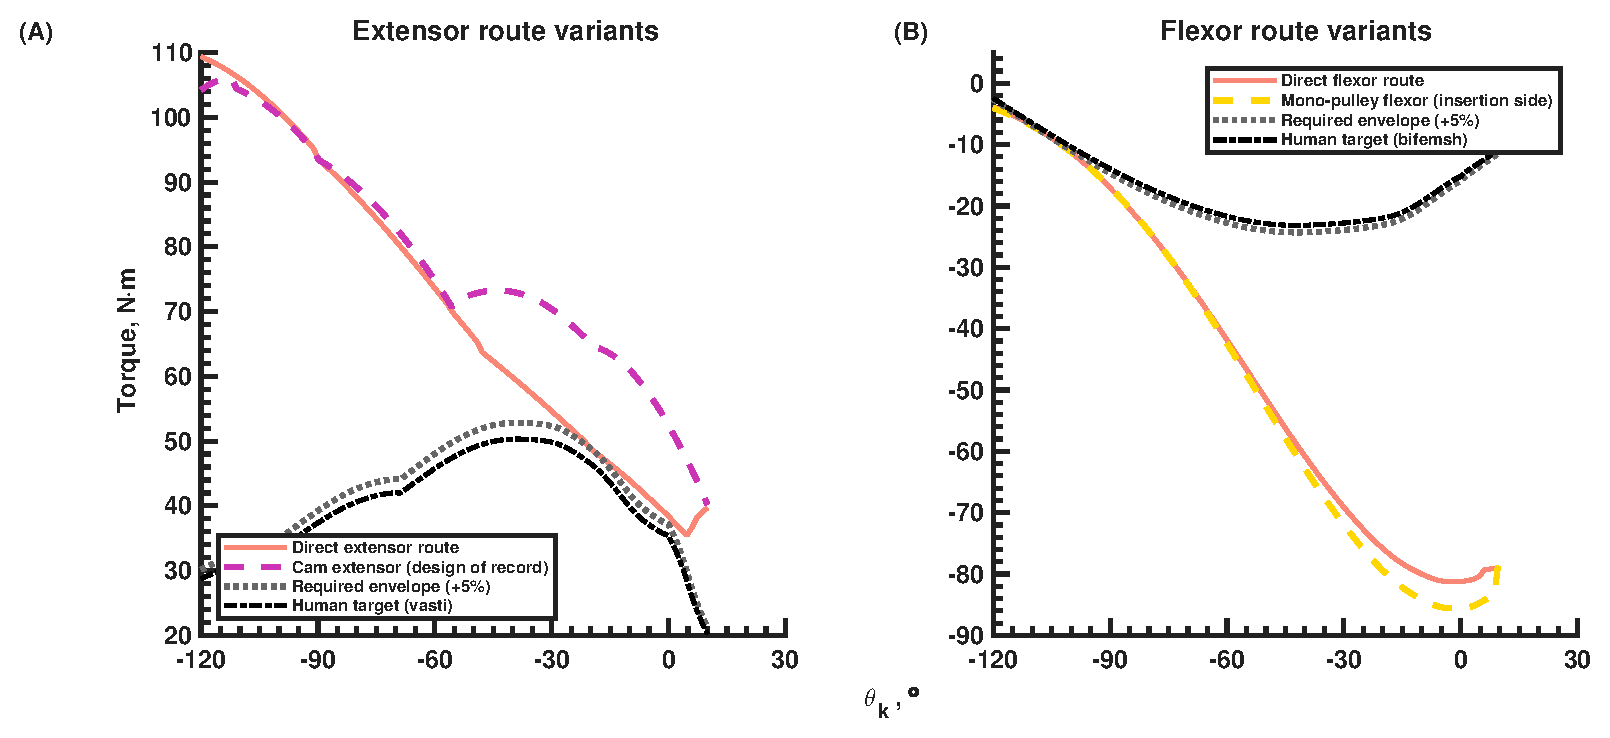
\includegraphics[width=1\textwidth]{Figures/RouteVariants_20261020.eps}
\end{center}
\caption{Predicted knee-axis torque of the redesigned route families against the human-scaled requirements. Knee angle is negative in flexion; extension torque is positive and flexion torque negative. \textbf{(A)} Extensor routes: the direct route and the cam design of record against the vasti requirement and its required \qty{5}{\percent} envelope. \textbf{(B)} Flexor routes: the direct two-BPA route and the mono-pulley variant on the insertion-side measure against the biceps femoris short-head requirement and its envelope.}\label{fig:RouteVariants}
\end{figure}

\begin{figure}[htbp]
\begin{center}
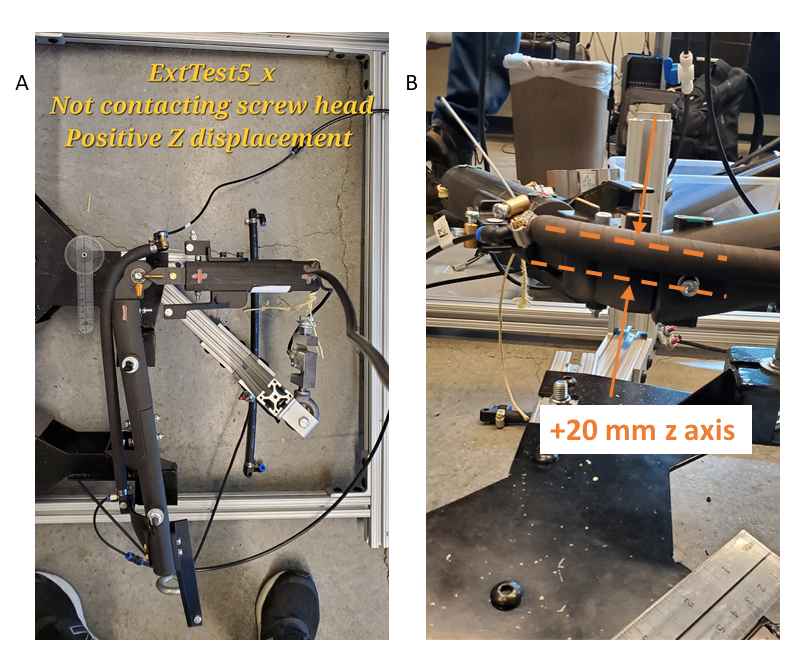
\includegraphics[width=1\textwidth]{Figures/extensor_misalign.png}
\end{center}
\caption{During extensor tests with the pinned knee using a tendon it was noticed that the actuator pathway was modeled to be anterior of the socket head cap screw that joins the femur body to the knee assembly. This slippage affects the muscle path and the moment arm. It was determined this caused a \qty{\pm20}{\milli\metre} $\hat{z}$ axis displacement. Test assembly is shown with \textbf{(A)} top down view and  \textbf{(B)} side view.}
\label{fig:extensor_misalign}
\end{figure}

\bibliography{BolenFrontiers22}









\subsection{Contact and Release Angles of the Wrapped Route}\label{app:contact_release}

The route-elimination rule that schedules the wrapped extensor route is a route-topology state machine rather than a shortest-path solver: the fully flexed route carries every candidate contact, and each contact is released at the first more-extended knee angle at which the straight chord between its surviving neighbors can replace it without entering the exclusion envelopes. This section states the calculation in generic terms, so that it applies to any wrapped actuator route on a rotating joint pair; the extensor route of Table~\ref{tab:RouteRedesign20} gives the cam-route example; its release schedule follows the same rule on the cam geometry.

The route is stored as a fixed number of rows $p_{1},\ldots,p_{9}$: rows $p_{1}$ through $p_{5}$ are femur-frame points, rows $p_{6}$ through $p_{9}$ are tibia-frame points, and the segment from $p_{5}$ to $p_{6}$ crosses from one body frame into the other. The endpoints $p_{1}$ and $p_{9}$ are the actuator origin and insertion, and they are always active. Each interior row is either active, a genuine wrap contact, or eliminated; an eliminated femur-side row repeats the preceding active femur row, and an eliminated tibia-side row repeats the neighboring active tibia row, so the route keeps a fixed size and its segment chain crosses the joint exactly once. Let $\mathcal{A}(\theta_{\mathbf{k}}) \subseteq \{2,\ldots,8\}$ denote the active interior rows at knee angle $\theta_{\mathbf{k}}$. The sweep over the design grid, here 100 poses from $\ang{-120}$ to $\ang{+10}$ at a spacing of \qty{1.31}{\degree}, proceeds from full flexion toward extension, each pose inherits the active set of the previous pose, and rows are only ever removed, so $\mathcal{A}$ shrinks monotonically as the knee extends.

At every pose, every active interior row is tested between its nearest active anchors,
\begin{equation}
i^{-}_{j} = \max\{i < j : i \in \mathcal{A} \cup \{1\}\}, \qquad
i^{+}_{j} = \min\{i > j : i \in \mathcal{A} \cup \{9\}\},
\label{eq:app_anchors}
\end{equation}
with the anchors expressed in the candidate's native frame through the per-angle joint transforms. Write $A$, $B$, and $C$ for the planar, sagittal positions of $p_{i^{-}_{j}}$, $p_{i^{+}_{j}}$, and $p_{j}$, and let $s(x, y)$ denote the signed angle from vector $x$ to vector $y$, positive counterclockwise, evaluated as a single $\operatorname{atan2}$ of the planar cross product and the dot product so that no principal-value seam can corrupt the comparison. The elimination margin of row $j$ is
\begin{equation}
\mu_{j}(\theta_{\mathbf{k}}) =
\begin{cases}
s\!\left(C - A,\; B - A\right), & j \leq 5,\\[4pt]
s\!\left(A - B,\; C - B\right), & j \geq 6,
\end{cases}
\label{eq:app_elim_margin}
\end{equation}
a signed angle between the through-contact leg and the bypass chord, measured in the native wrap sense of the candidate's side of the crossing segment; the two cases differ only in that sense of rotation, because the femur-side contacts turn the route one way around the distal femur and the tibia-side contacts turn it the opposite way around the proximal tibia. The rotation rule releases the contact once the margin turns positive, the orientation at which the chord, rather than the contact, provides the outer boundary of the route on that side. The gate is opened slightly early,
\begin{equation}
\mu_{j}(\theta_{\mathbf{k}}) > -\Delta, \qquad \Delta = \qty{1.5}{\degree},
\label{eq:app_rotation_gate}
\end{equation}
as a release hysteresis: in the last poses before the contact becomes collinear with its chord, the computed moment arm of the wrapping segment collapses, and releasing the contact slightly before that orientation, with the collision gate below still controlling validity, removes the artifact without changing the route family.

Opening the rotation gate is necessary but not sufficient. A removal additionally requires the straight bypass chord $\overline{AB}$ to clear the exclusion envelopes of the candidate's side,
\begin{equation}
\operatorname{dist}\!\left(\overline{AB}_{\mathrm{trim}},\, \mathcal{E}_{j}\right) \;\geq\; g, \qquad g = \qty{0.5}{\mm},
\label{eq:app_bypass_gate}
\end{equation}
where $\operatorname{dist}$ is the planar clearance between the trimmed chord and the envelope and tangency is allowed. The chord is trimmed by \qty{2}{\mm} at each end, capped at \qty{45}{\percent} of its length, because a legitimate contact departs from the clearance boundary itself. On the femur side the envelopes $\mathcal{E}_{j}$ are the femoral-cylinder clearance circle, the condyle clearance polygon, and the femoral-wall span; on the tibia side they are the two tibial-cylinder clearance circles and the wall band between them. Every envelope is the normal offset of a bone profile by the fully inflated BPA radius $R_{\mathrm{BPA}}$,
\begin{equation}
\mathbf{q}(\vartheta) = \mathbf{e}(\vartheta) + R_{\mathrm{BPA}}\,\hat{\mathbf{n}}(\vartheta),
\label{eq:app_offset_curve}
\end{equation}
where $\mathbf{e}(\vartheta)$ traces the physical profile and $\hat{\mathbf{n}}(\vartheta)$ is its outward normal; the offset curve shares the tangent of the physical profile, its radius of curvature is $\rho(\vartheta) = \rho_{\mathrm{phys}}(\vartheta) + R_{\mathrm{BPA}}$, and the candidate contact positions themselves are seeded at tangent points of this curve. Because the envelopes are drawn at the fully inflated radius while the routed BPA is contracted at the release angles, each envelope radius may be relaxed by $\rho = \qty{3}{\mm}$ inside the gate, floored at the bone profile plus \qty{0.5}{\mm}; a rotation-gate opening that still fails the relaxed collision gate indicates that the seed placement, not the gate, must move.

At the first pose of the sweep, full flexion, the seed route is settled to a fixpoint: every contact whose two gates already open there is removed, and removals repeat until no further gate opens, so that the sweep starts from a valid topology; a colinearity guard may additionally remove a seed contact that starts the sweep already aligned with its neighbors, and its tolerance is zero in the design of record, so every seed row of Table~\ref{tab:RouteRedesign20} starts active. At every later pose at most one contact is released: if several rows open both gates in the same pose, the row with the largest elimination margin, the one whose rotation rule is most decisively open, is released first, and the remaining rows are retested at the next pose. The release angle of row $j$ is recorded as the first grid pose at which the row is inactive. The activation angle is read from the same record with the sweep reversed, as the last pose at which the row is active, which is the pose at which the contact re-engages when the route is driven from extension toward flexion.

The same active-set record drives the geometric bend measure that scales the fictive-strain wrapping loss of Equations~\eqref{eq:deltaL} and~\eqref{eq:x3} inside the stiffness-aware force balance. Each wrap family, the femoral-cylinder contact, the femoral-condyle curve, the tibial contact curve, and the crossing-point curve at the ICR, contributes an arc length over its effective radius, and the total
\begin{equation}
b(\theta_{\mathbf{k}}) = \sum_{f} R_{f}(\theta_{\mathbf{k}})\, \alpha_{f}(\theta_{\mathbf{k}})
\label{eq:app_bend_measure}
\end{equation}
is the bend signal handed to the force model. Each family's turn angle $\alpha_{f}$ ramps with knee angle between the two route-state events that bound it, holding zero before the first event and its plateau after the second, so the topology state and the bending signal are two readings of one record. The formulation is joint-agnostic: it requires only a fixed route representation with one crossing segment, per-angle transforms between the two body frames, and clearance envelopes on each side, so it carries unchanged to the other wrapped routes of this program.


\clearpage
\subsection{Configuration-Survey Coordinates and Actuator Sizes}

\begin{table}[htbp]
\centering
\caption{Degrees of freedom and nominal BPA sizes in the 27-site configuration survey. Diameter follows the inherited robot sizing rule and is retained on the updated side. At nominal \qty{40}{\mm} sites, the baseline instead uses four parallel \qty{20}{\mm} BPAs; other baseline sites use one actuator of the listed diameter. The two coordinate columns identify the graded surface, rather than every coordinate a multiarticular route could cross.}
\label{tab:survey_dofs_sizes}
\begingroup\small\renewcommand{\arraystretch}{1.1}
\begin{tabular}{@{}lllll@{}}
\toprule
\textbf{Site} & \textbf{Primary DoF} & \textbf{Secondary DoF} & \textbf{Dia. (mm)} & \textbf{Baseline (mm)} \\
\midrule
ercspn\_r & lumbar ext. & lumbar bend. & 40 & 4$\times$20 \\
intobl\_r & lumbar ext. & lumbar bend. & 20 & 1$\times$20 \\
extobl\_r & lumbar ext. & lumbar bend. & 20 & 1$\times$20 \\
bifemlh\_r & knee & hip flex. & 20 & 1$\times$20 \\
semimem\_r & knee & hip flex. & 40 & 4$\times$20 \\
sar\_r & knee & hip flex. & 10 & 1$\times$10 \\
tfl\_r & knee & hip flex. & 10 & 1$\times$10 \\
rect\_fem\_r & knee & hip flex. & 20 & 1$\times$20 \\
grac\_r & knee & hip flex. & 10 & 1$\times$10 \\
bifemsh\_r & knee & hip flex. & 20 & 1$\times$20 \\
vas\_int\_r & knee & hip flex. & 40 & 4$\times$20 \\
soleus\_r & ankle & knee & 40 & 4$\times$20 \\
med\_gas\_r & ankle & knee & 40 & 4$\times$20 \\
lat\_gas\_r & ankle & knee & 20 & 1$\times$20 \\
tib\_post\_r & subtalar & ankle & 40 & 4$\times$20 \\
tib\_ant\_r & ankle & subtalar & 20 & 1$\times$20 \\
per\_brev\_r & subtalar & ankle & 10 & 1$\times$10 \\
per\_long\_r & subtalar & ankle & 20 & 1$\times$20 \\
per\_tert\_r & subtalar & ankle & 10 & 1$\times$10 \\
flex\_dig\_r & MTP & ankle & 10 & 1$\times$10 \\
flex\_hal\_r & MTP & ankle & 10 & 1$\times$10 \\
ext\_dig\_r & MTP & ankle & 10 & 1$\times$10 \\
ext\_hal\_r & MTP & ankle & 10 & 1$\times$10 \\
glut\_max\_r & hip flex. & hip add. & 40 & 4$\times$20 \\
add\_mag\_r & hip add. & hip flex. & 40 & 4$\times$20 \\
iliacus\_r & hip flex. & hip add. & 20 & 1$\times$20 \\
psoas\_r & hip flex. & hip add. & 20 & 1$\times$20 \\
\bottomrule
\end{tabular}
\endgroup
\end{table}
\end{document}
